
\newcommand{\figscale}{0.24}

\begin{subfigure}[b]{\figscale\textwidth}
      \begin{tikzpicture}[scale=\figscale]
        \node[anchor=south east,inner sep=0] at (0,0) {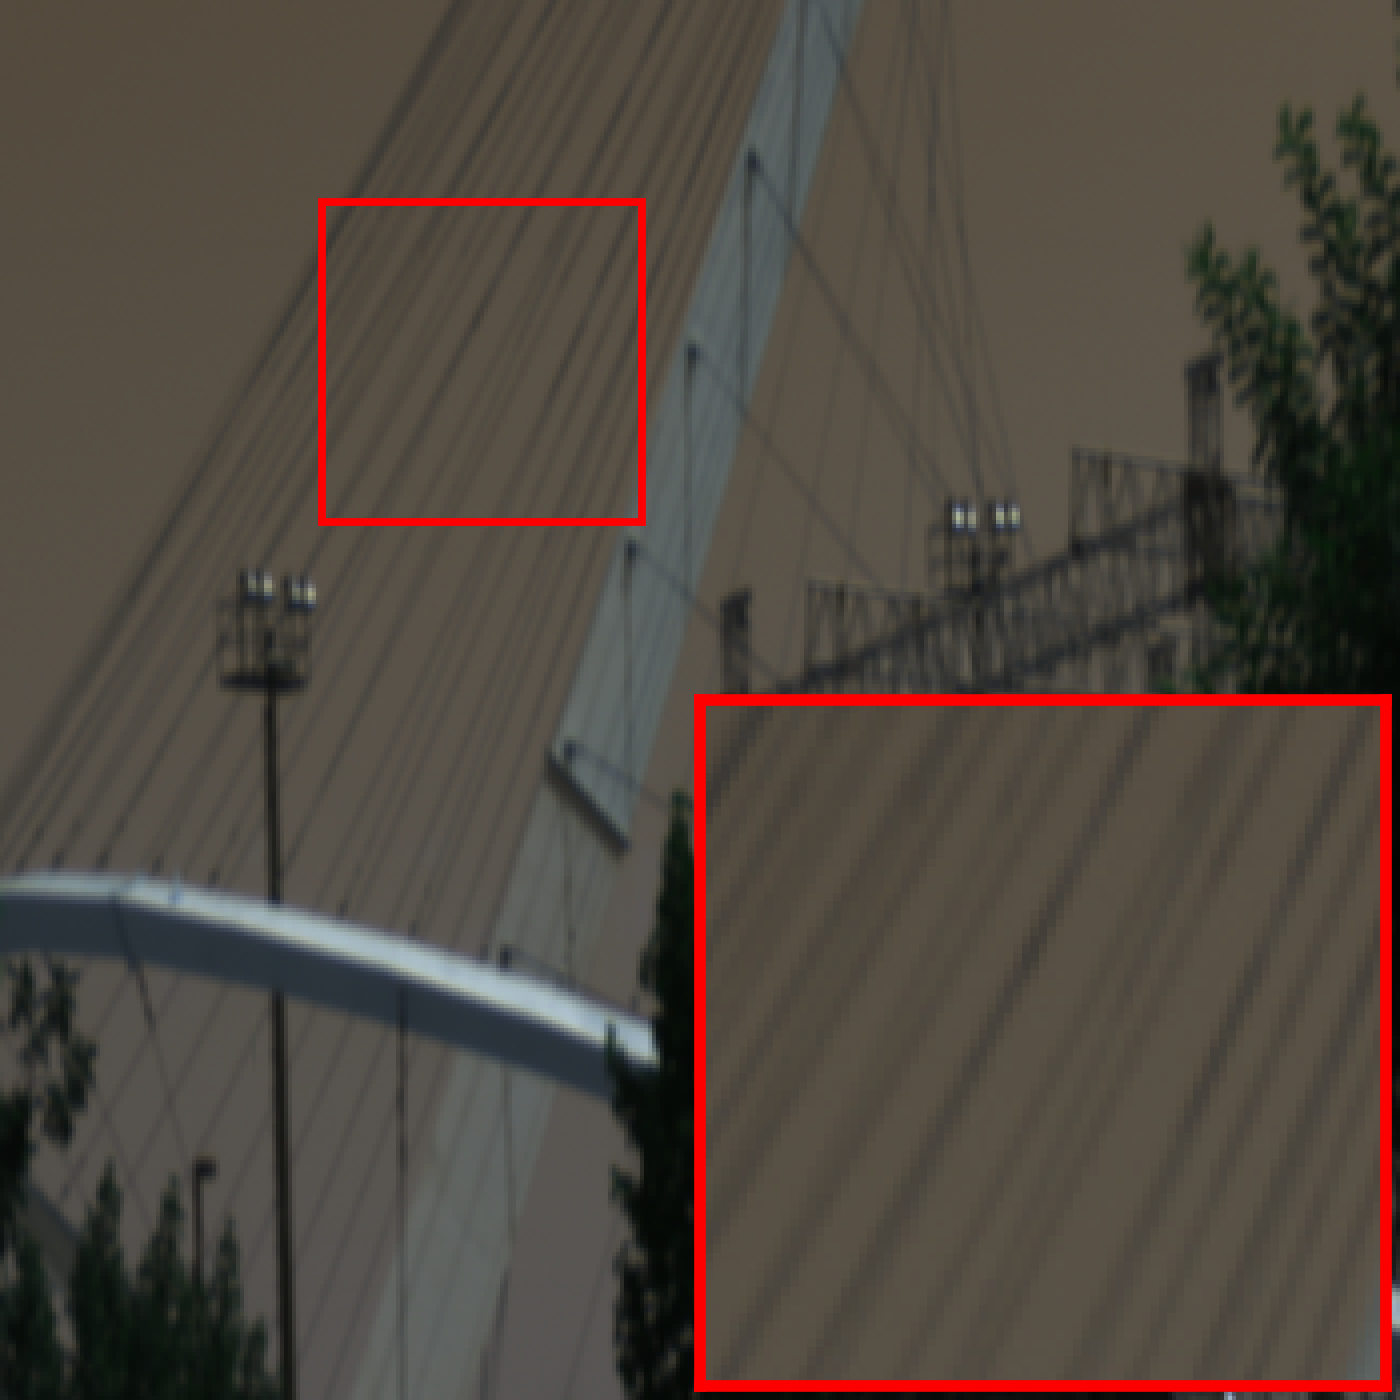
\includegraphics[width=\textwidth]{fichiers_latex/Chap1/figs/stripes/clean.png}};
      \end{tikzpicture}
   \caption{Groundtruth}
\end{subfigure}
\hfill
\begin{subfigure}[b]{\figscale\textwidth}
      \begin{tikzpicture}[scale=\figscale]
        \node[anchor=south east,inner sep=0] at (0,0) {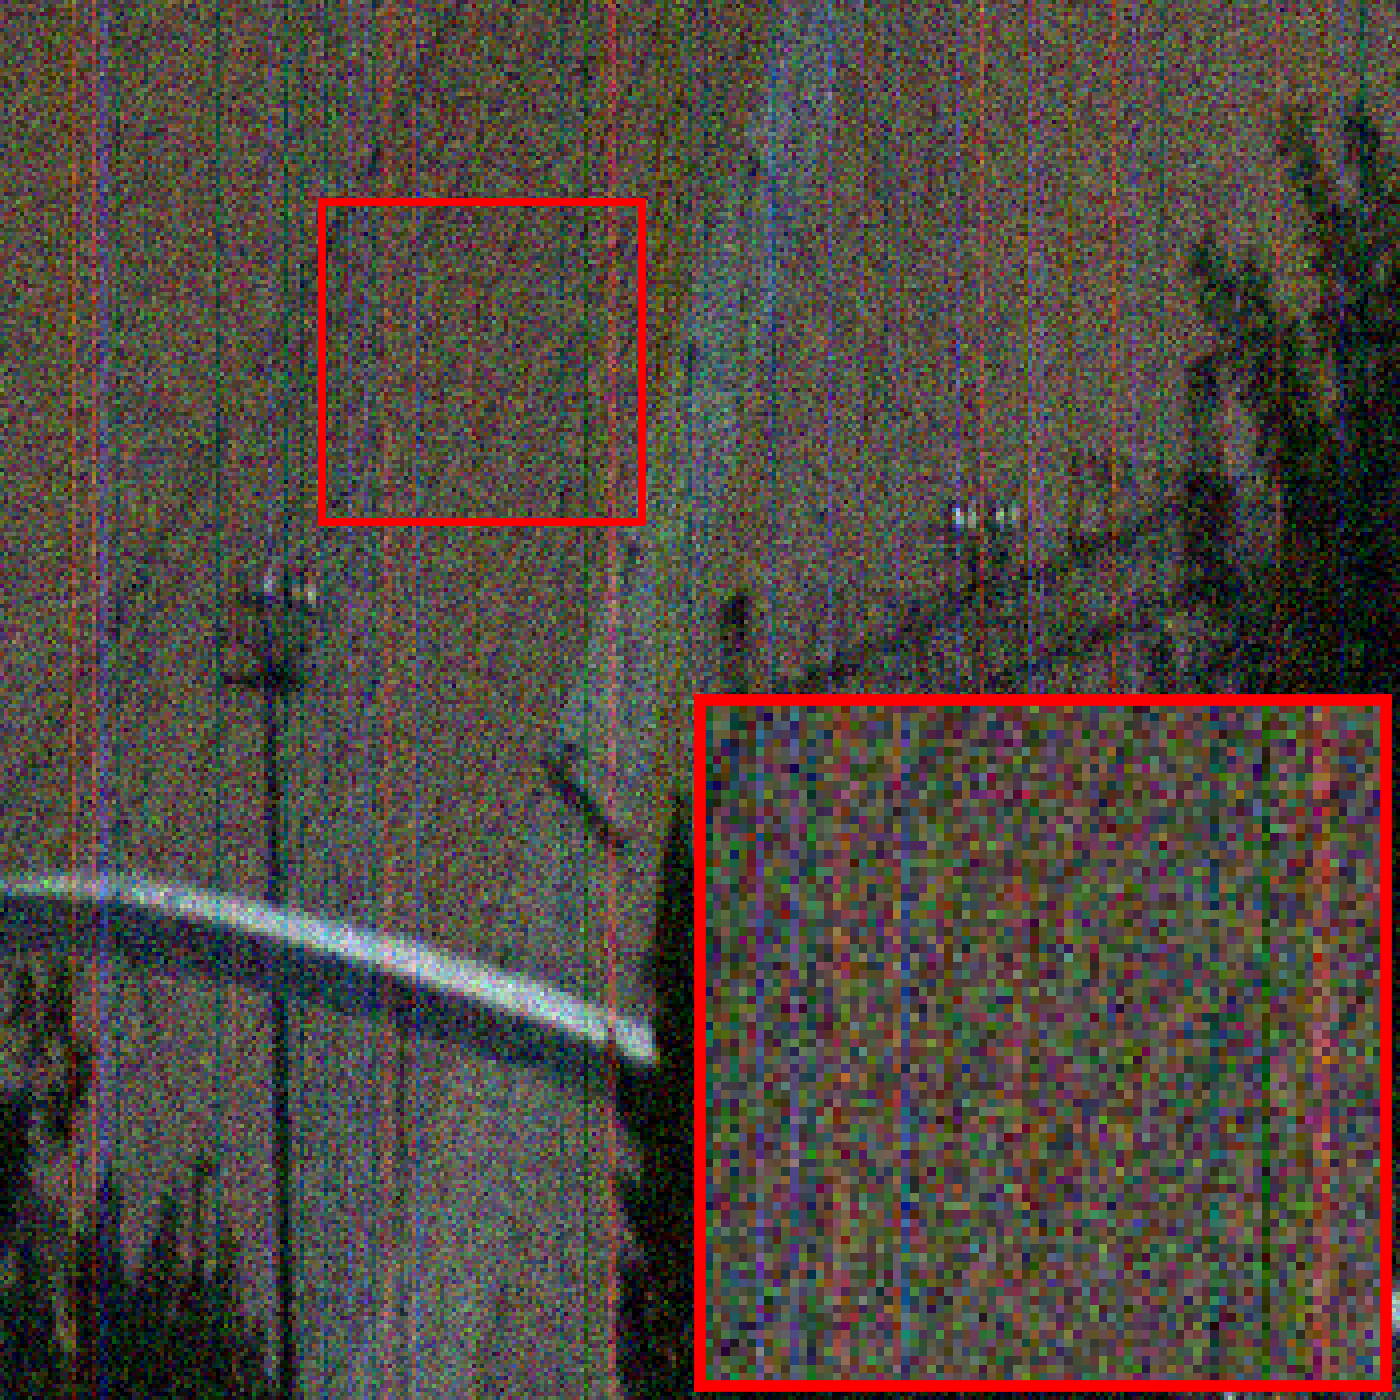
\includegraphics[width=\textwidth]{fichiers_latex/Chap1/figs/stripes/in.png}};
      \end{tikzpicture}
   \caption{Noisy}
\end{subfigure}
\hfill
\begin{subfigure}[b]{\figscale\textwidth}
      \begin{tikzpicture}[scale=\figscale]
        \node[anchor=south east,inner sep=0] at (0,0) {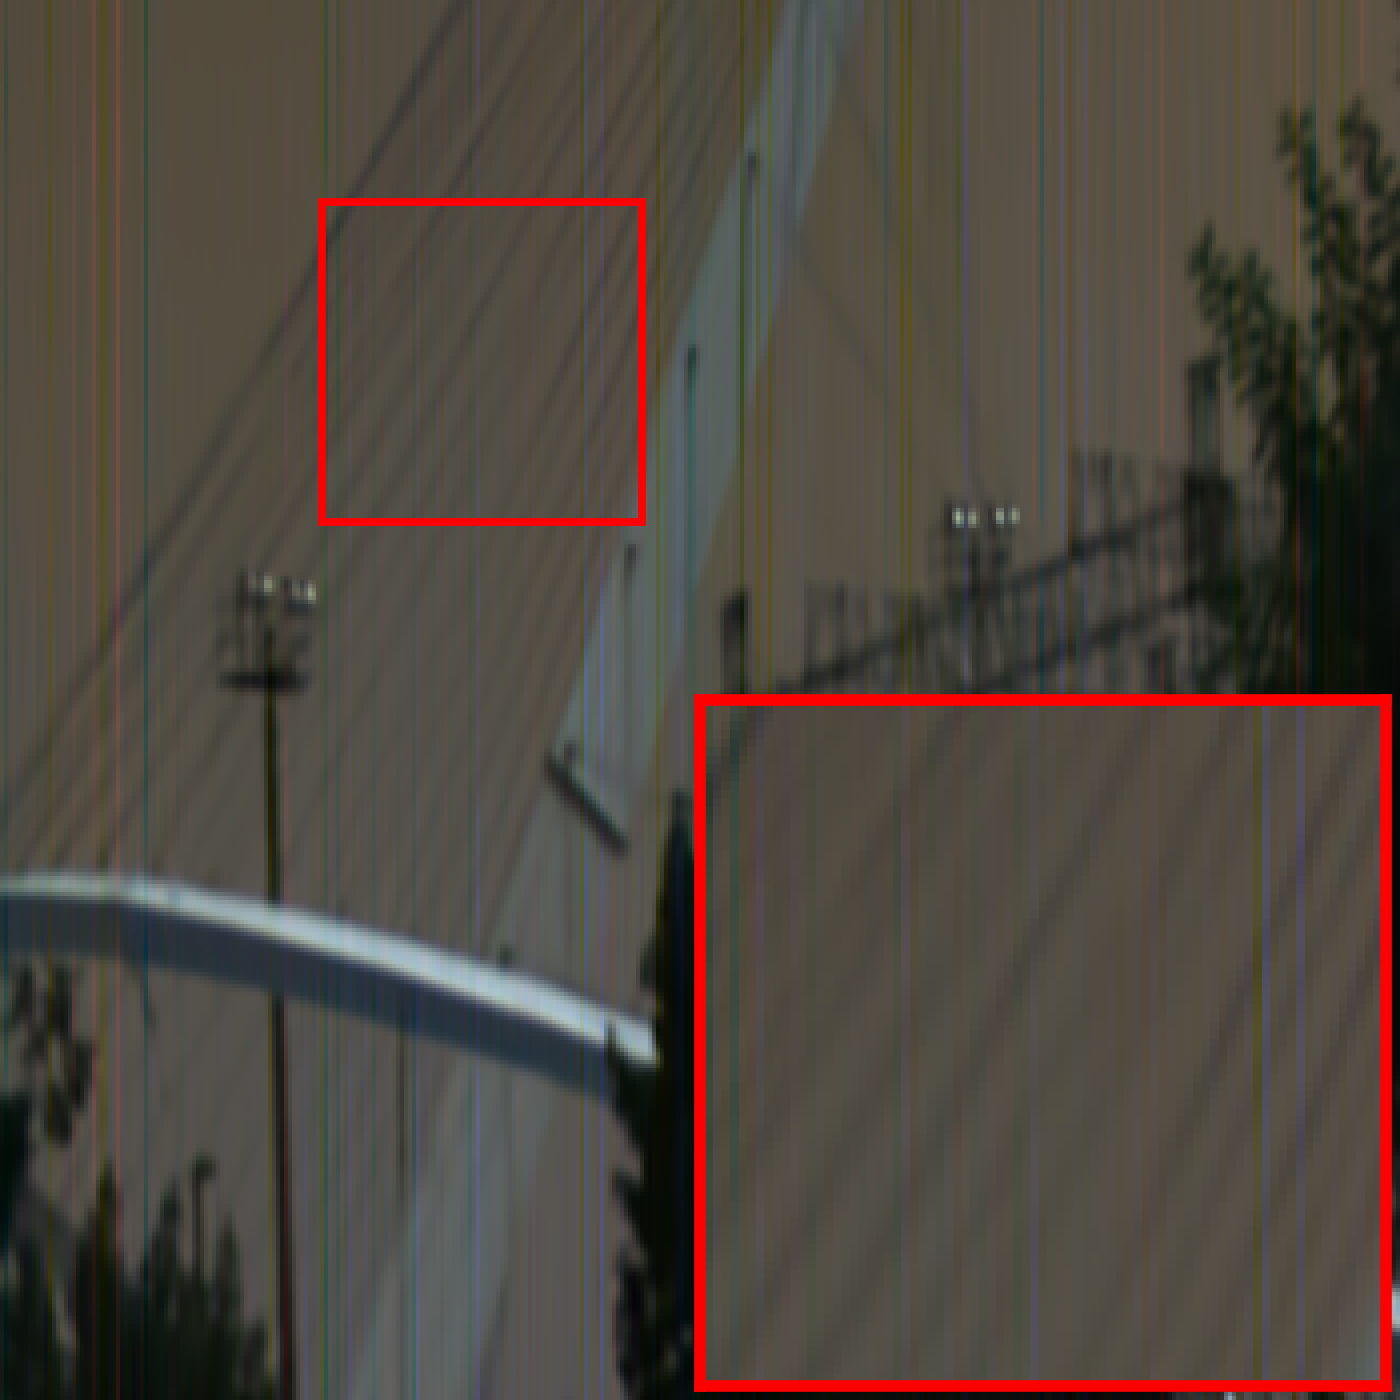
\includegraphics[width=\textwidth]{fichiers_latex/Chap1/figs/stripes/llrt.png}};
      \end{tikzpicture}
   \caption{LLRT}
\end{subfigure}
\hfill
\begin{subfigure}[b]{\figscale\textwidth}
      \begin{tikzpicture}[scale=\figscale]
        \node[anchor=south east,inner sep=0] at (0,0) {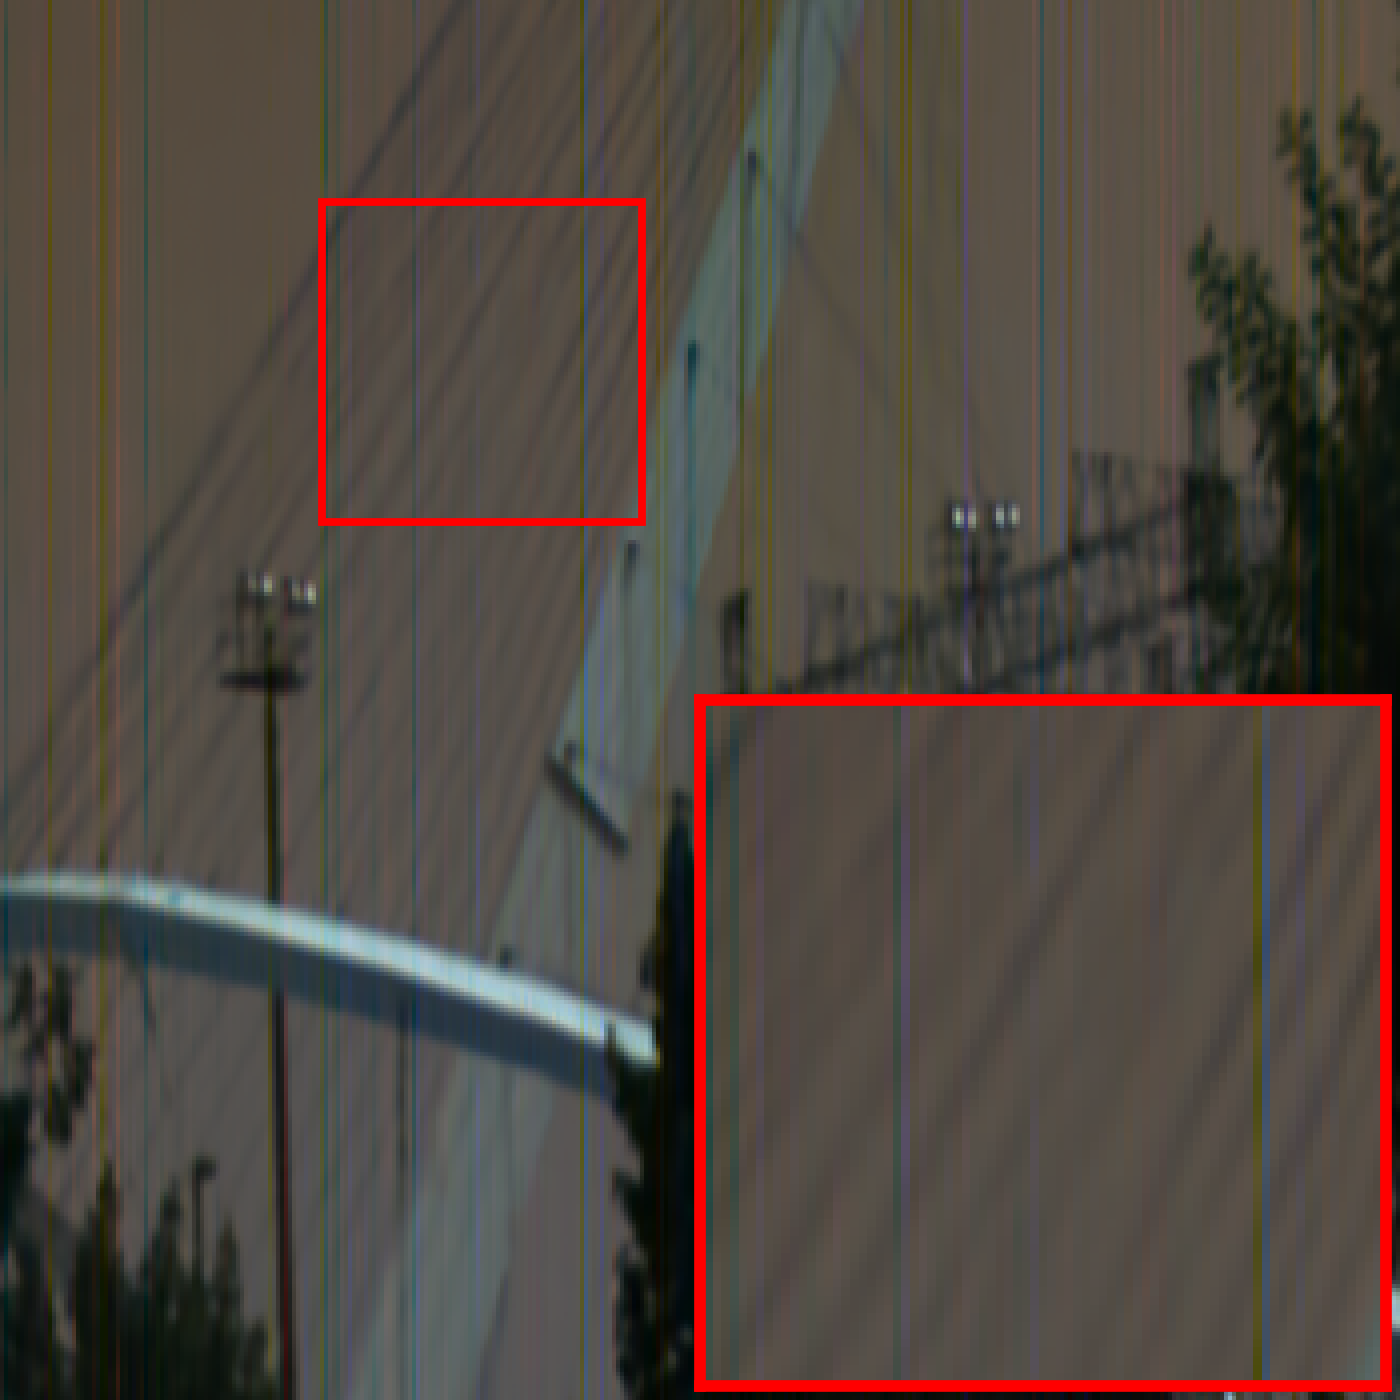
\includegraphics[width=\textwidth]{fichiers_latex/Chap1/figs/stripes/ngmeet.png}};
      \end{tikzpicture}
   \caption{NGMeet}
\end{subfigure}
\\
\begin{subfigure}[b]{\figscale\textwidth}
      \begin{tikzpicture}[scale=\figscale]
        \node[anchor=south east,inner sep=0] at (0,0) {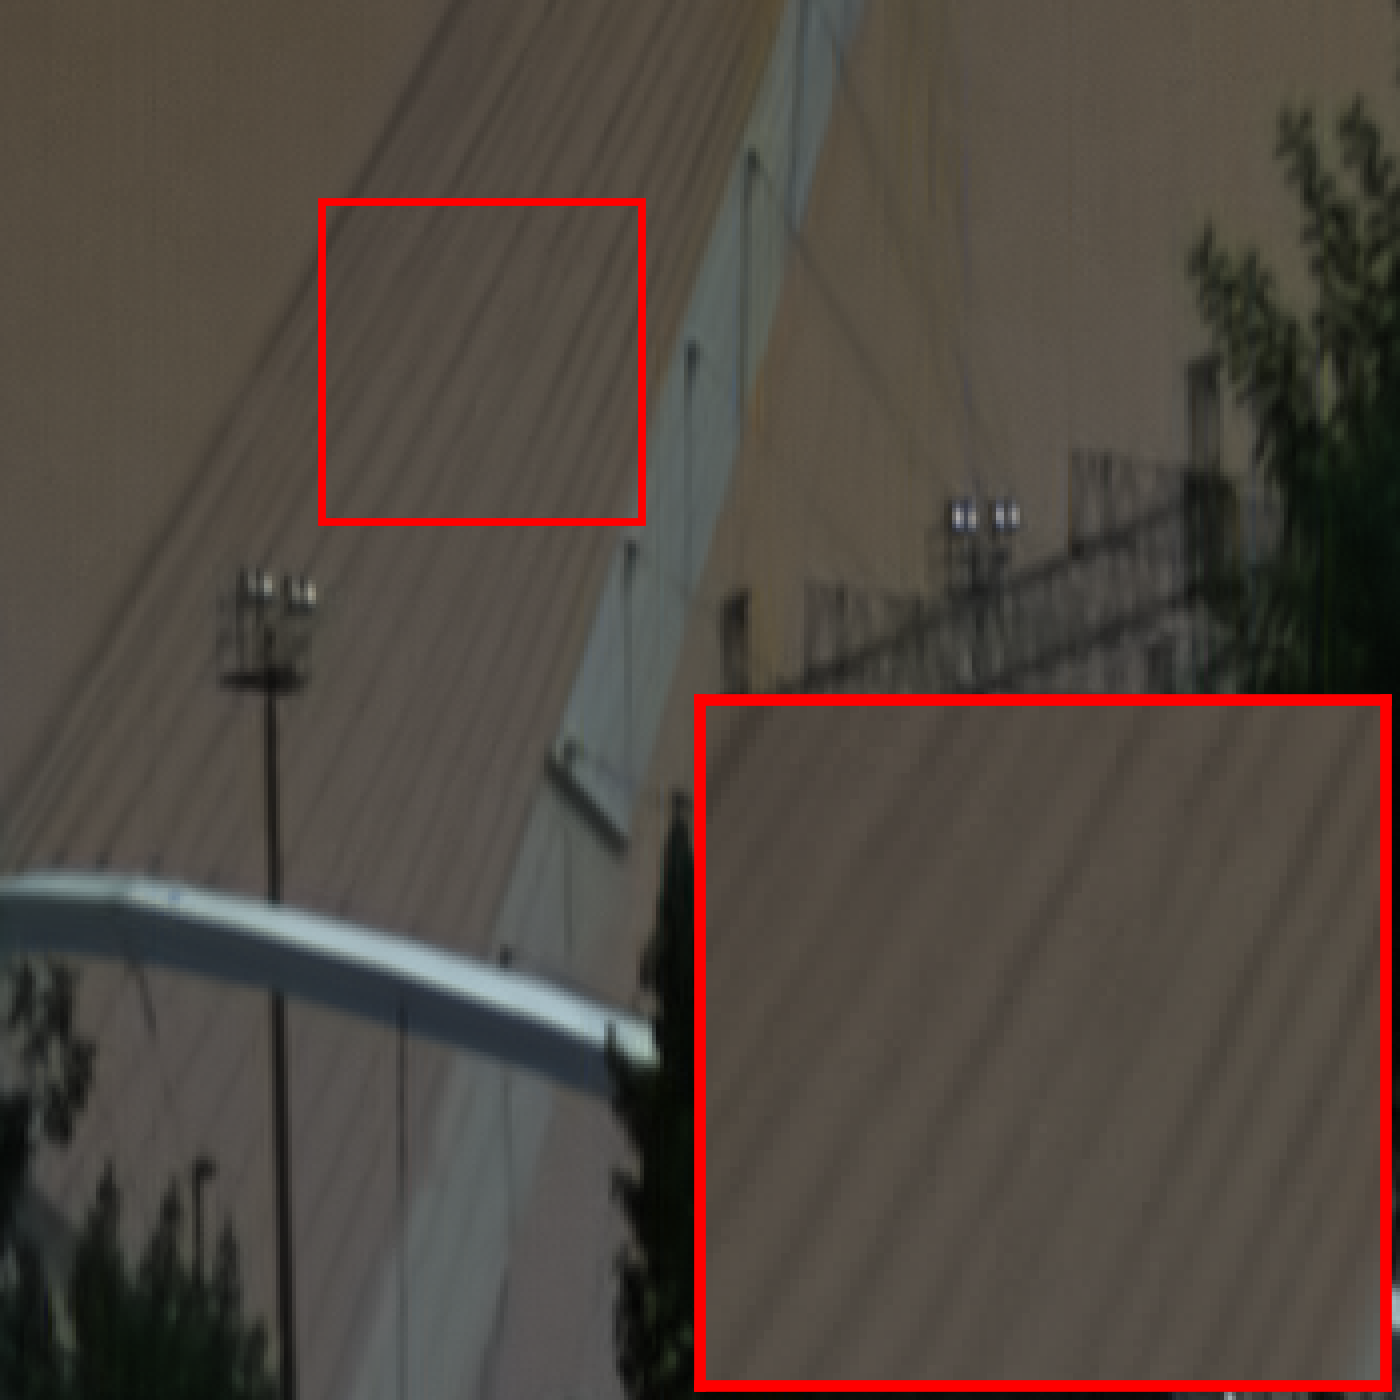
\includegraphics[width=\textwidth]{fichiers_latex/Chap1/figs/stripes/glf.png}};
      \end{tikzpicture}
   \caption{GLF}
\end{subfigure} 
\hfill
\begin{subfigure}[b]{\figscale\textwidth}
      \begin{tikzpicture}[scale=\figscale]
        \node[anchor=south east,inner sep=0] at (0,0) {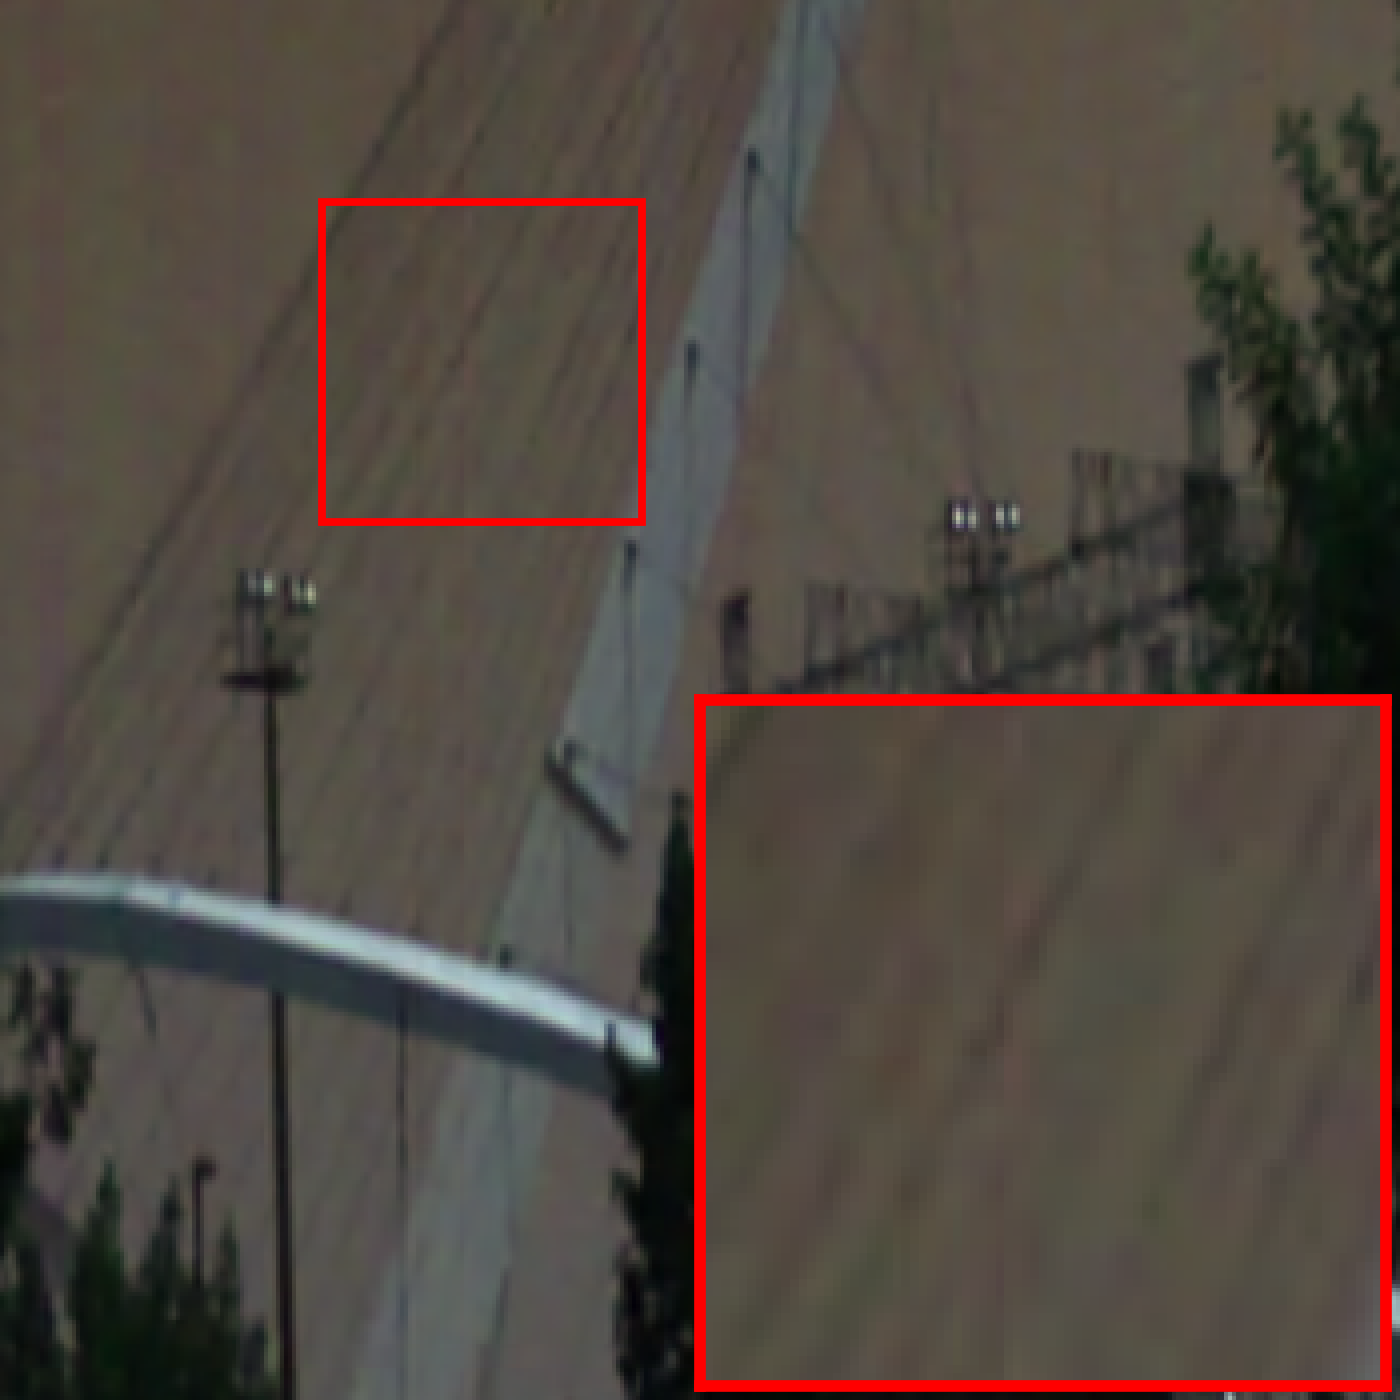
\includegraphics[width=\textwidth]{fichiers_latex/Chap1/figs/stripes/smds.png}};
      \end{tikzpicture}
   \caption{SMDS-Net}
\end{subfigure}
\hfill
\begin{subfigure}[b]{\figscale\textwidth}
      \begin{tikzpicture}[scale=\figscale]
        \node[anchor=south east,inner sep=0] at (0,0) {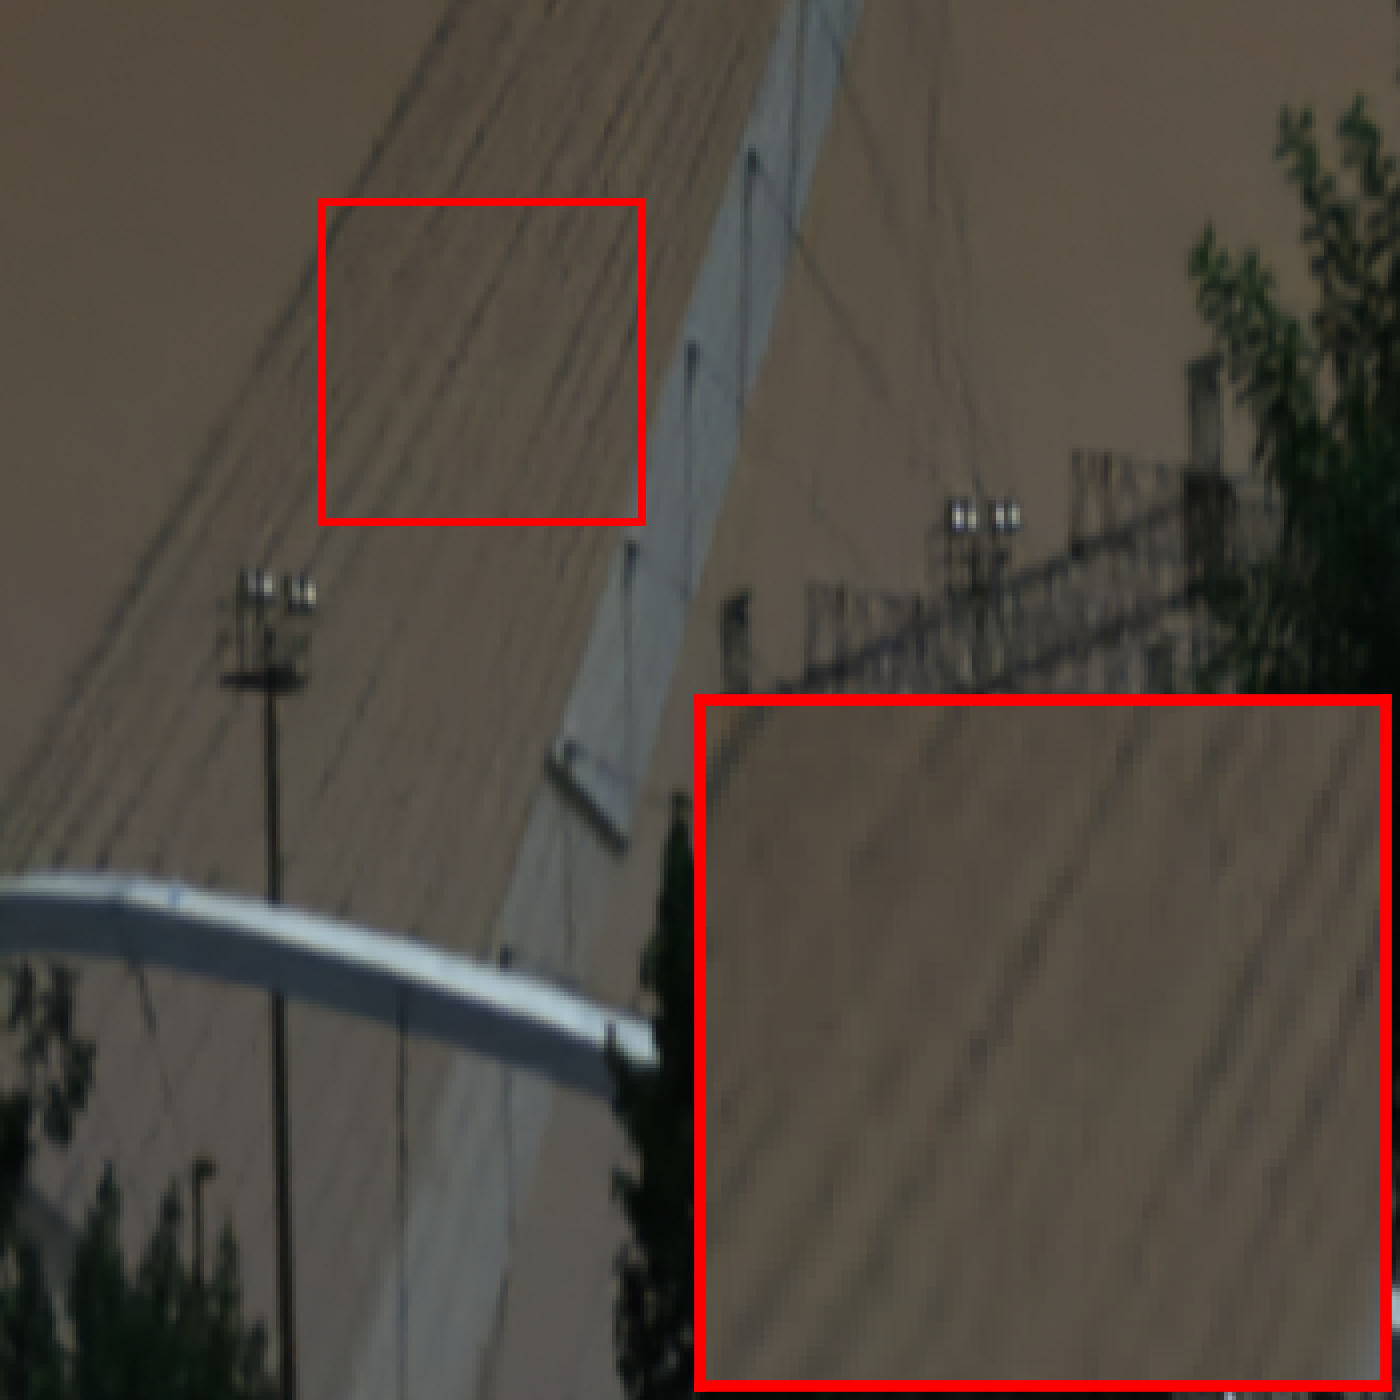
\includegraphics[width=\textwidth]{fichiers_latex/Chap1/figs/stripes/qrnn.png}};
      \end{tikzpicture}
   \caption{QRNN3D}
\end{subfigure}
\hfill
\begin{subfigure}[b]{\figscale\textwidth}
      \begin{tikzpicture}[scale=\figscale]
        \node[anchor=south east,inner sep=0] at (0,0) {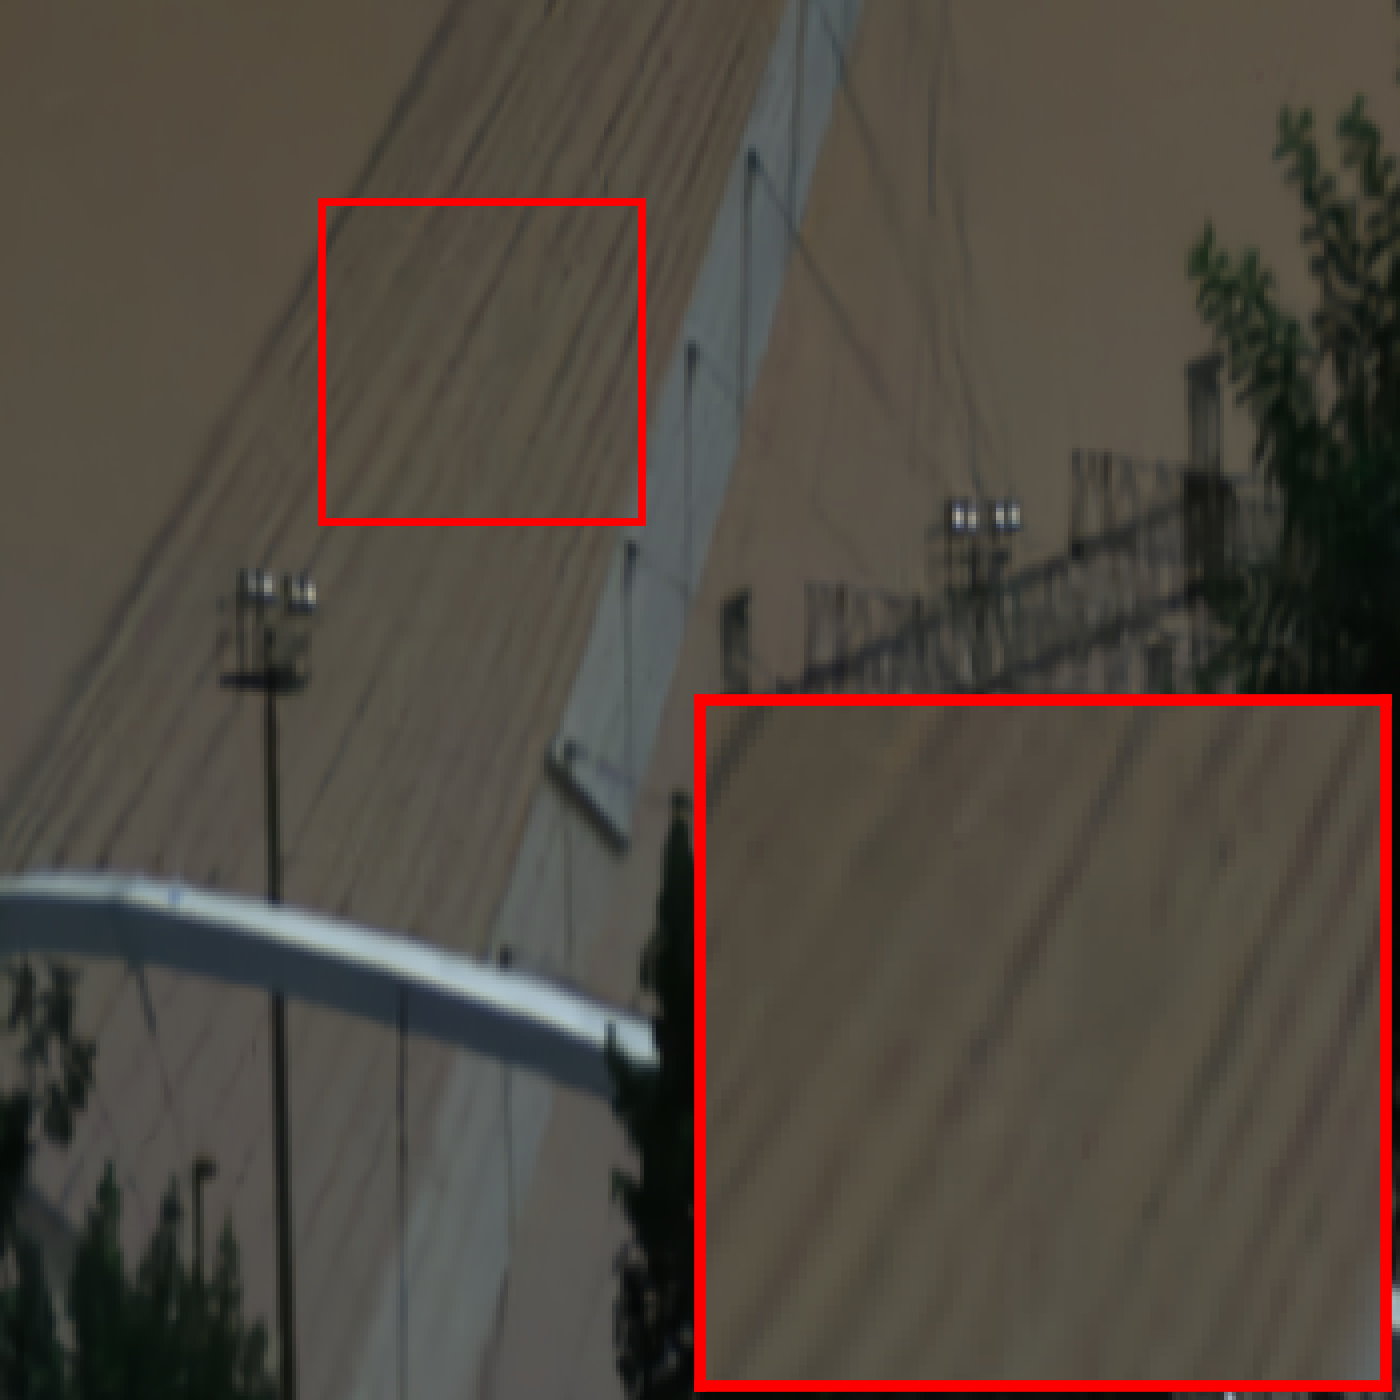
\includegraphics[width=\textwidth]{fichiers_latex/Chap1/figs/stripes/t3sc.png}};
      \end{tikzpicture}
   \caption{T3SC}
\end{subfigure}

